\section{Validation and Testing}\label{sec:chapter-7}

\subsection{Test strategy and evidence boundaries}

Validation combines saved evaluation outputs, regression-test source, and an existing device-and-backend test record. The report does not claim that these suites were newly rerun during preparation. The functional record is dated 15 September 2026 and describes an iPhone simulator with local Node, PostgreSQL, and Docker recommendation services. That provides useful integration evidence, while leaving physical-device behaviour, production configuration, and full automated native screen coverage unresolved.

Different checks address different failure classes. Ranking metrics quantify agreement with authored relevance labels. Explicit-exclusion tests check whether declared policy is preserved. Cryptographic tests examine round trips and tampering failures. API checks examine ownership and accepted formats. Native checks address module availability, secure key storage, restart persistence, and connectivity. A good score in one layer cannot substitute for a missing check in another, so the conclusions preserve these evidence boundaries.

\subsection{Journal-free ranking benchmark}

The journal-free ONNX run was generated on 18 September 2026 using hybrid-v4, the MiniLM ONNX backend, 30 scenarios, ten repeats per approach, and seed 42. Four approaches were compared: random ranking, semantic text similarity, rules with eligibility, and the hybrid. All deduplicate and honour explicit exercise exclusions, but random and text-only do not apply the same suitability rules as rules and hybrid. This is a comparison of complete approaches, not a controlled ablation isolating one component.

Relevance is defined as an authored label of at least two. Precision@4 divides relevant returned items by four, penalising unfilled slots. NDCG@4 uses graded gains and rank discounts to compare the returned ordering with an ideal ordering. Negative labels contribute zero gain but are also reported through a separate violation measure. Fill rate helps reveal systems that avoid violations simply by returning nothing. Bootstrap intervals resample the 30 scenario means; they estimate variation within this dataset rather than clinical or population uncertainty.

\begingroup
\small\setstretch{1.08}
\setlength{\tabcolsep}{4pt}
\setlength{\TableInnerWidth}{\dimexpr\linewidth-24pt\relax}
\begin{longtable}{@{}>{\raggedright\arraybackslash}p{0.340\TableInnerWidth} >{\raggedright\arraybackslash}p{0.200\TableInnerWidth} >{\raggedright\arraybackslash}p{0.200\TableInnerWidth} >{\raggedright\arraybackslash}p{0.260\TableInnerWidth}@{}}
\caption{Saved journal-free ONNX benchmark, 30 authored scenarios. Violation percentages represent negative benchmark labels, not measured adverse outcomes.}\label{tab:table-3}\\
\toprule
\textbf{Approach} & \textbf{Precision@4} & \textbf{NDCG@4} & \textbf{Negative-label items} \\
\midrule\endfirsthead
\multicolumn{4}{l}{\textit{Table \thetable\ continued}}\\
\toprule
\textbf{Approach} & \textbf{Precision@4} & \textbf{NDCG@4} & \textbf{Negative-label items} \\
\midrule\endhead
\midrule\multicolumn{4}{r}{\textit{Continued on next page}}\\\endfoot
\bottomrule\endlastfoot
Random & 48.50\% & 0.4315 & 5.17\% \\ \addlinespace[4pt]
MiniLM text similarity & 71.67\% & 0.6602 & 1.67\% \\ \addlinespace[4pt]
Rules + eligibility & 73.33\% & 0.7244 & 2.50\% \\ \addlinespace[4pt]
Hybrid & 77.50\% & 0.7387 & 3.33\% \\ \addlinespace[4pt]
\end{longtable}
\endgroup

The hybrid returned an average of 3.1 relevant items per four. Its precision exceeded rules by 4.17 percentage points and NDCG by 0.0143. Those improvements are modest and should be read alongside the higher negative-label rate. Text-only recorded fewer negative-labelled selections in this suite. Figure~\ref{fig:productionchart} includes quality and warm timing, making the trade-offs visible rather than selecting only the strongest hybrid metric. No statistical significance or clinical superiority is inferred from the point estimates.

\begin{figure}[htbp]
\centering
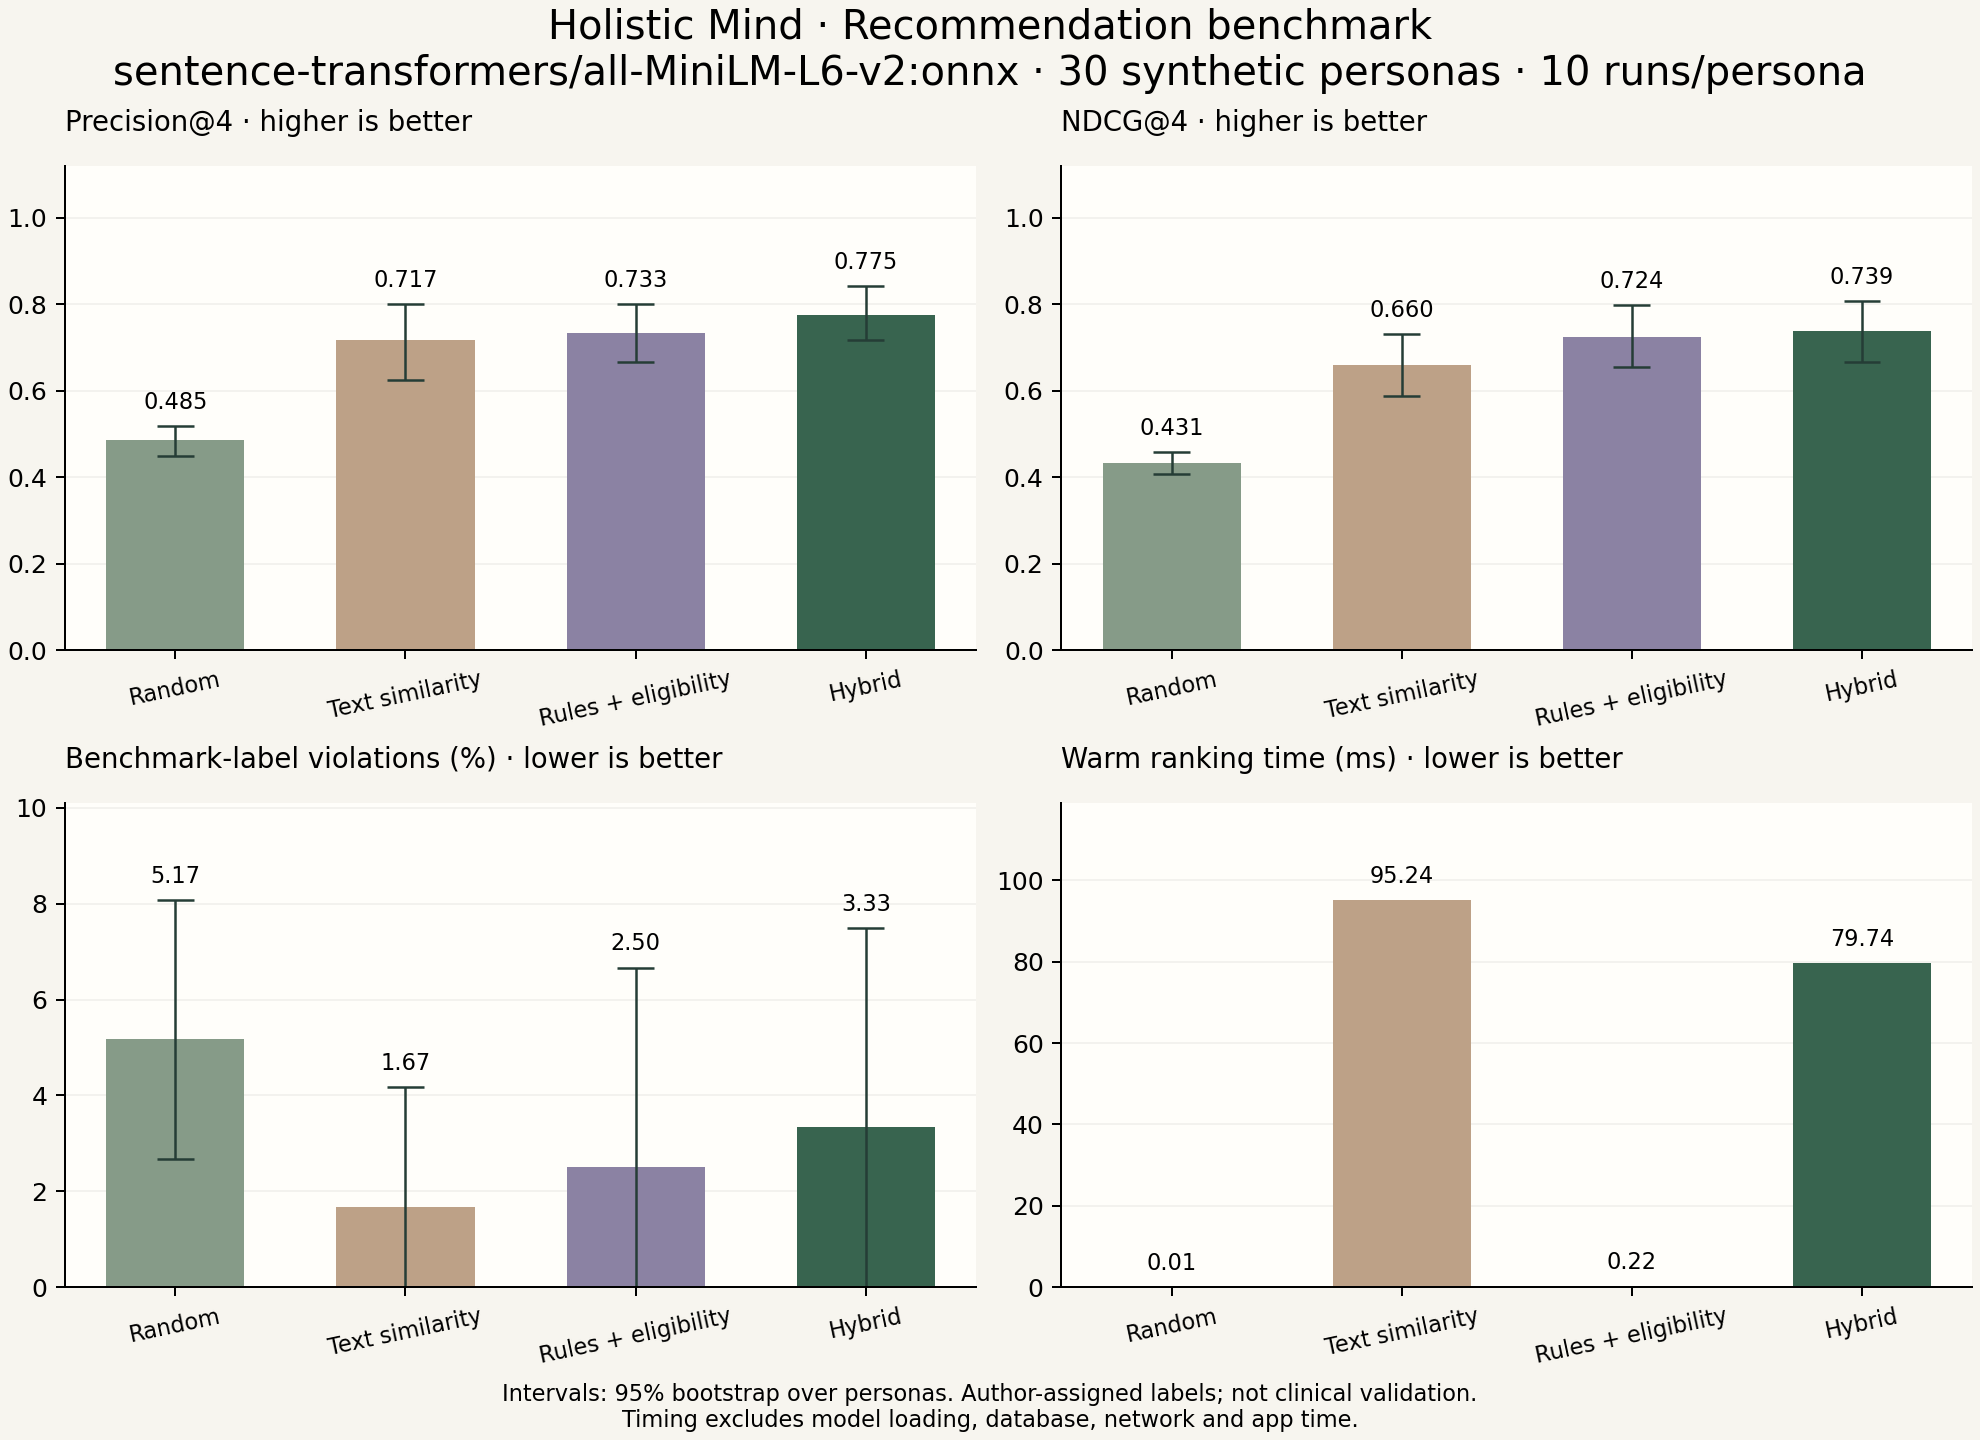
\includegraphics[width=\linewidth,height=0.62\textheight,keepaspectratio]{figures/productionchart.png}
\caption[Journal-free ONNX benchmark results]{Existing project benchmark chart for journal-free ONNX evaluation. Error bars are bootstrap intervals over authored scenarios; timing excludes startup, database, HTTP, and mobile rendering.}
\label{fig:productionchart}
\end{figure}
\FloatBarrier

\subsection{Comfort restrictions and unresolved cases}

The separate comfort suite contains eight selected variants with declared choices, including individual restrictions and combinations. All approaches recorded zero explicit exclusion violations with full top-four fill in these selected cases. Hybrid precision was 90.62\% and NDCG was 0.7441, while text-only NDCG was higher at 0.7885. These figures should not be compared directly with the 30-scenario benchmark because the comfort cases are a selected stress suite, sometimes derived from the same source persona.

\begin{figure}[htbp]
\centering
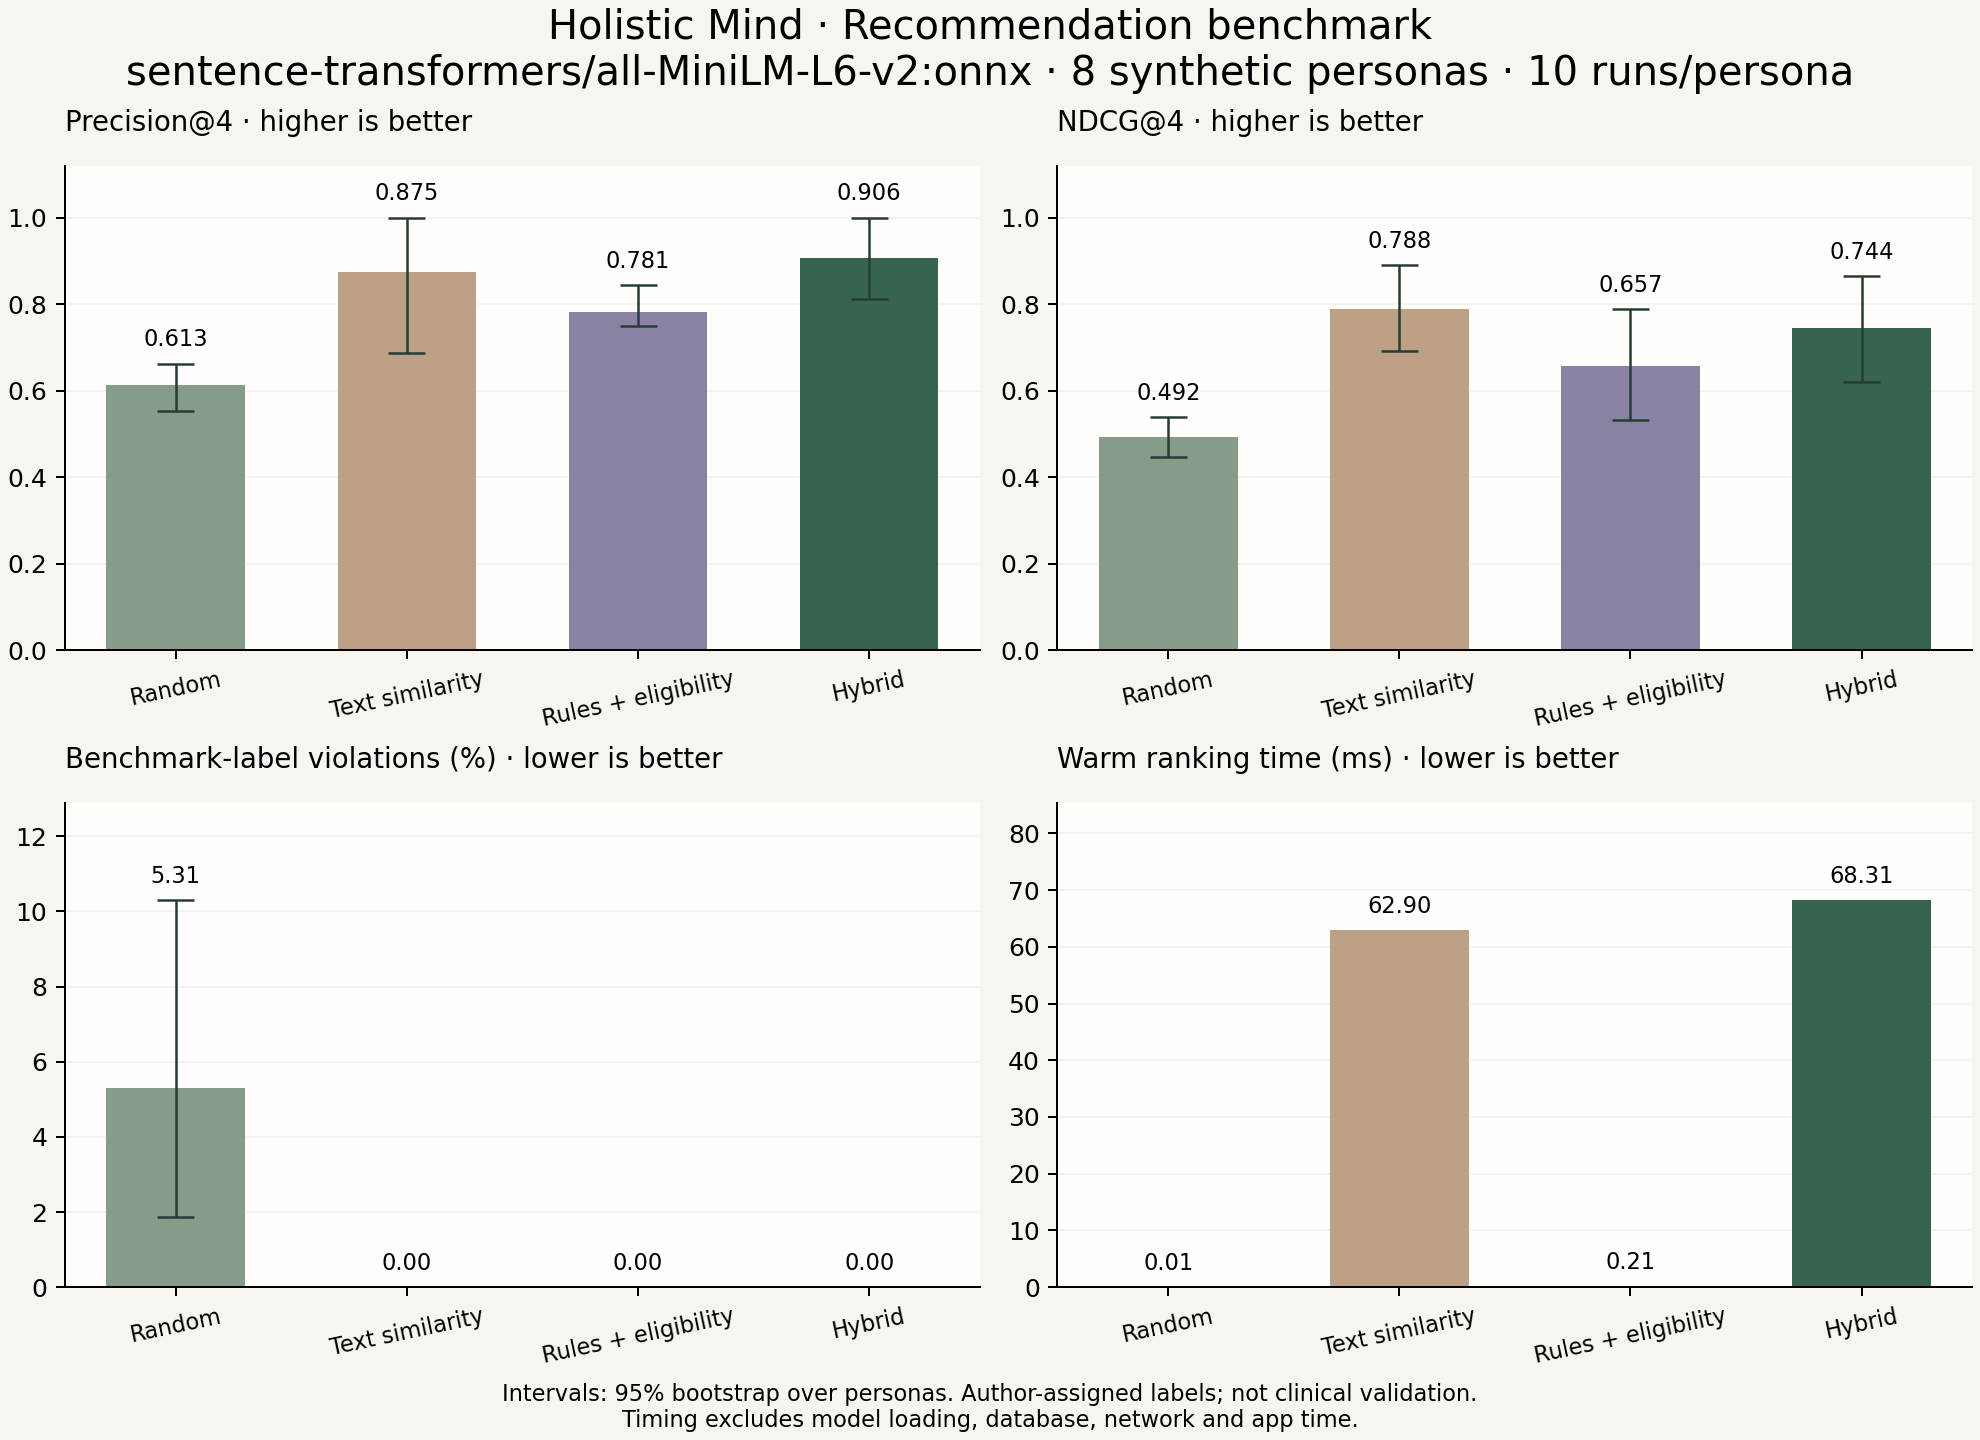
\includegraphics[width=\linewidth,height=0.62\textheight,keepaspectratio]{figures/comfortchart.png}
\caption[Explicit-comfort ONNX benchmark results]{Existing comfort-suite ONNX chart, eight selected scenarios. The suite tests declared restrictions; it does not establish detection of unspoken concerns or representative user performance.}
\label{fig:comfortchart}
\end{figure}
\FloatBarrier

Three original cases remain informative. One describes touch aversion only in synthetic journal text, another describes head or eye scanning discomfort without a corresponding declared choice, and another negatively labels body scanning without a matching metadata restriction. Current production cannot read the journals, and none of these failures should be hidden by inventing preferences after the fact. Separate variants demonstrate that explicit choices trigger exclusions, while the original labels remain unchanged. Independent review is needed for disputed suitability judgments.

\subsection{Documented functional checks}

The September test record reports successful native encryption/\allowbreak{}decryption, Nepali and emoji round trips, recovery-key verification, rejection of different-account decryption, SecureStore readback, and key persistence after terminating and relaunching the application. Live backend checks used temporary synthetic accounts to verify vault setup, encrypted save/\allowbreak{}read, duplicate retry behaviour, account separation, legacy migration, plaintext rejection, comfort-choice persistence, and a live hybrid-v4 ONNX response. Temporary fixtures were cleaned up after those checks.

The same record documents problems with a missing native cryptography module, a simulator build lacking keychain entitlements, and an outdated running recommender container. Rebuilding the native app with the required module and signing, then rebuilding the recommender, resolved those recorded issues. This illustrates why source correctness alone is insufficient for native integration. A library can exist in JavaScript while being absent from the installed binary. Release validation must therefore include the actual installed application and service versions.

\subsection{Metrics, timing, and uncertainty}

Precision and NDCG answer related but different questions. Precision measures the proportion of the requested four slots occupied by exercises with labels of at least two. NDCG rewards stronger labels placed earlier. Recall divides relevant returns by all relevant labelled items for that scenario. MRR concerns the position of the first relevant item. Coverage and category diversity describe catalogue use rather than whether any individual user benefits. Reading these measures together prevents one favourable result from standing in for the complete recommendation experience.

The benchmark's negative-label measure is named safety\_violation\_rate in the saved output, but its meaning is disagreement with authored negative labels. It is not an observed adverse-event rate. Explicit-exclusion violations are a separate property: an exercise can violate an authored label even when the user supplied no corresponding restriction. Conversely, a strongly relevant exercise may be excluded by a user's expressed preference. That is why the comfort suite's unchanged ideal relevance labels can limit interpretation of recall and NDCG.

Timing describes warm, in-process ranking. The saved production chart reports mean times of approximately 0.01 ms for random, 95.24 ms for semantic-only, 0.22 ms for rules, and 79.74 ms for hybrid. The hybrid's lower time than text-only in this run is not proof of universal speed superiority; candidate filtering and measurement variation affect the workload. Model load, tokeniser setup, database queries, HTTP transport, and mobile rendering are excluded. User-perceived delay requires a separate end-to-end measurement.

Bootstrap intervals reflect uncertainty over these authored scenarios. They do not compensate for a biased catalogue, uncertain labels, or a missing held-out dataset. Some comfort cases share a source persona, limiting independence further. The correct conclusion is that the saved runs make technical comparison transparent and reproducible under their recorded conditions. A stronger research claim requires additional data and a design that distinguishes development choices from final evaluation.

\subsection{Verification matrix and regression priorities}

\begingroup
\small\setstretch{1.08}
\setlength{\tabcolsep}{4pt}
\setlength{\TableInnerWidth}{\dimexpr\linewidth-24pt\relax}
\begin{longtable}{@{}>{\raggedright\arraybackslash}p{0.220\TableInnerWidth} >{\raggedright\arraybackslash}p{0.260\TableInnerWidth} >{\raggedright\arraybackslash}p{0.260\TableInnerWidth} >{\raggedright\arraybackslash}p{0.260\TableInnerWidth}@{}}
\caption{Verification evidence by system layer. These are recorded or source-observed results, not newly rerun application tests for this report.}\label{tab:table-4}\\
\toprule
\textbf{Layer} & \textbf{Evidence source} & \textbf{Supported conclusion} & \textbf{Outstanding check} \\
\midrule\endfirsthead
\multicolumn{4}{l}{\textit{Table \thetable\ continued}}\\
\toprule
\textbf{Layer} & \textbf{Evidence source} & \textbf{Supported conclusion} & \textbf{Outstanding check} \\
\midrule\endhead
\midrule\multicolumn{4}{r}{\textit{Continued on next page}}\\\endfoot
\bottomrule\endlastfoot
Mobile types and exports & September/\allowbreak{}October change records & Recorded checks passed & Production-signed device release \\ \addlinespace[4pt]
Comfort policy & Shared mapping; regression suite & Declared exclusions exercised & Usability of preference wording \\ \addlinespace[4pt]
Journal crypto/\allowbreak{}API & Synthetic tests and live API record & Round trips; ownership; migration & Independent security assessment \\ \addlinespace[4pt]
Native key storage & 15 September simulator record & Key persists after restart & Physical-device recovery/\allowbreak{}reinstall \\ \addlinespace[4pt]
Ranking quality & 18 September saved ONNX runs & Authored relevance comparison & Unseen scenarios; expert labels \\ \addlinespace[4pt]
Administration/\allowbreak{}content & Source and September review & Managed publication implemented & Editorial and load validation \\ \addlinespace[4pt]
Provider login & Source and 3 October change record & Configuration and readiness work & Complete current Google login \\ \addlinespace[4pt]
Usability/\allowbreak{}effectiveness & Earlier proposed protocol & Research design available & Consented participant evaluation \\ \addlinespace[4pt]
\end{longtable}
\endgroup

The regression plan should focus on failures with consequences across layers. A declared exclusion should survive backend mapping, Python filtering, diversity selection, and local fallback. An account change should clear the active journal session. A repeated encrypted save should not create duplicate entries. A migration retry should not overwrite an already encrypted record. Recommendation feedback should reject references that do not belong to an owned returned request. These checks test requirements rather than duplicating implementation details.

More recent features require particular care when interpreting older results. The September native record concerns the tested journal modules and synthetic fixtures at that time. It cannot automatically validate later attachment composition or reorganised security screens. The October build/\allowbreak{}export and journal-test record adds evidence for recent changes, but still identifies hands-on recovery UI and physical-device Google sign-in as pending. A versioned verification matrix makes these differences visible to a reviewer.

\subsection{Planned user acceptance evaluation}

The original minimum-five-participant study remains a useful formative proposal. Participants would complete representative tasks, give practice-relevance ratings, and discuss perceived control and confusion. Standard SUS scoring can be used if the instrument is administered without changing its measurement assumptions; an adapted questionnaire should be reported as adapted rather than presented as a standard SUS score. A small study would identify issues and guide iteration, not establish population effectiveness.

A random comparator requires additional care because the software's purpose includes restrictions. A fair user-study comparator should randomise within the same eligible, independently reviewed pool rather than deliberately offer excluded practices. The current offline baseline's omission of suitability rules is acceptable as a clearly documented diagnostic comparison, but does not justify presenting inappropriate content to participants. Appendix C specifies how a future protocol could separate relevance, comfort, task completion, and optional qualitative feedback.
